]%Este trabalho está licenciado sob a Licença Creative Commons Atribuição-CompartilhaIgual 3.0 Não Adaptada. Para ver uma cópia desta licença, visite http://creativecommons.org/licenses/by-sa/3.0/ ou envie uma carta para Creative Commons, PO Box 1866, Mountain View, CA 94042, USA.

%\documentclass[main.tex]{subfiles}
%\begin{document}

\chapter{Solução de equações de uma variável}\index{equações!de uma variável}

Neste capítulo buscaremos aproximações numéricas para a solução de equações de uma variável real. Observamos que resolver uma dada equação de uma variável real é equivalente a encontrar os zeros de uma função apropriada. Com isso, iniciamos este capítulo discutindo sobre condições de existência de raízes de funções reais. Então, apresentamos o método da bisseção como uma primeira abordagem numérica para encontrar zeros de funções.

Em seguida, exproramos uma outra abordagem via iteração do ponto fixo. Desta, obtemos o método de Newton, para o qual discutimos sua aplicação e convergência. Por fim, apresentamos o método das secantes como uma das possíveis variações do método de Newton.

\section{Existência de raízes reais}\index{função!raiz}\index{função!zero}

Podemos utilizar o teorema do valor intermediário para determinar a existência de raiz real em um intervalo.

\begin{teo}[Teorema do Valor Intermediário]
Se $f:[a,b]\to\mathbb{R}$ é um função contínua e $K$ for um número entre $f(a)$ e $f(b)$, então existe $c\in(a,b)$ para o qual $f(c)=K$.
\end{teo}

\begin{figure}[h!]
  \centering
  \includegraphics[scale=0.5]{./cap_equacao1d/pics/teorema_do_valor_intermediario/teorema_do_valor_intermediario.eps}
  \caption{Teorema do valor intermediário}
  \label{fig:teorema_do_valor_intermediario}
\end{figure}

Em particular, se $f(a)>0$ e $f(b)<0$, então $0\in [f(b),f(a)]$ e podemos garantir a existência de $c\in(a,b)$ tal que $f(c)=0$, i.e. existe uma raiz no intervalo $(a,b)$. A mesma afirmação é válida se $f(a)<0$ e $f(b)>0$. Em outras palavras, o Teorema do Valor Intermediário afirma que uma função contínua não pode mudar de sinal sem passar por zero.

\begin{ex}
Mostre que existe pelo menos uma solução da equação $e^x=x+2$ no intervalo $(-2,0)$.

De fato, se tomarmos $f(x)=e^x-x-2$, então $f(0)=1-2<0$ e $f(-2)=e^{-2}+2-2>0$. Pelo teorema do valor intermediário, existe $c\in(-2,0)$ tal que $f(c)=0$, ou seja, existe pelo menos uma solução nesse intervalo.
\end{ex}
Quando procuramos aproximações para raízes de funções, precisamos inicialmente isolar cada raiz em um intervalo onde a raiz é única. Ou seja, precisamos garantir a existência e a unicidade da raiz dentro daquele intervalo.

Para garantirmos que exista uma única raiz num intervalo é necessário que a função troque de sinal e seja monótona neste intervalo.

\begin{teo}
Se $f:[a,b]\to\mathbb{R}$ é um função diferenciável, $f(a)\cdot f(b)<0$ e $f'(x)>0$ (ou $f'(x)<0$) para $x\in(a,b)$, então existe uma única raiz $c$ em $(a,b)$.
\end{teo}

Em outras palavras, se a função corta o eixo $x$ e é sempre crescente (ou sempre decrescente), então a raiz é única.
\begin{ex}
Observamos que existe uma única solução da equação $e^x=x+2$ no intervalo $(-2,0)$. A existência foi estabelecida no exemplo anterior. Para garantir a unicidade, observe que $f'(x)=e^x-1$ e, portanto, $f'(x)<0$ para $x\in(-2,0)$. Logo a raiz é única.

\ifisscilab
Podemos inspecionar o comportamento da função $f(x)= e^x - x - 2$ e de sua derivada fazendo seus gráficos no Scilab. Para tanto, podemos fazer o seguinte teste:
\begin{verbatim}
-->x = linspace(-2,0,50);
-->deff('y = f(x)','y=exp(x)-x-2')  // define f
-->plot(x,f(x))                     // grafico de f
-->deff('y = fl(x)','y=exp(x)-1')   // a derivada
-->plot(x,fl(x))                    // grafico de f'
\end{verbatim}
\fi
\end{ex}

\section*{Exercícios}

\begin{Exercise}Mostre que a equação
  \begin{equation*}
    \ln(x)+x^3-\frac{1}{x}=10  
  \end{equation*}
possui uma única solução positiva. Faça o gráfico e observe.
\end{Exercise}

\begin{Exercise} Use o teorema do valor intermediário para mostrar que o erro absoluto ao aproximar a raiz da função $f(x)=e^x-x-2$ por $\overline{x}=-1,841$ é menor que $10^{-3}$.
\end{Exercise}

\begin{Exercise} Aplique o teorema do valor intermediário a um intervalo adequado e mostre que o erro absoluto associado à aproximação $1,962$ para a solução  exata $x^*$ de:
  \begin{equation*}
    e^x+\sin (x) +x = 10  
  \end{equation*}
é inferior a $10^{-4}$.
\end{Exercise}

\begin{Exercise}\label{existe_unica} Mostre que a equação
  \begin{equation*}
    \ln(x)+x-\frac{1}{x}=v
  \end{equation*}
possui uma solução para cada $v$ real e que esta solução é única.
\end{Exercise}


\section{Método da bisseção}\index{método!da bisseção}

Suponha que a função $f:[a,b]\to\mathbb{R}$ seja contínua e que $f(a)\cdot f(b)<0$, ou seja, $f(x)$ possui uma raiz no intervalo. A idéia do método da bisseção é de assumir o ponto médio $p$ do intervalo, i.e. $p=\frac{a+b}{2}$, como primeira aproximação para a raíz de $f(x)$. Uma segunda aproximação é obtida analisando o sinal da função nos pontos $x=a$, $x=p$ e $x=b$. Se $f(a)\cdot f(p)<0$, então a raiz está no intervalo $[a, p]$, senão, a raiz está no intervalo $[p, b]$ (veja Figura \ref{fig:bisection_scheme}). Então, escolhemos o intervalo que contém a raiz e tomamos o seu ponto médio como nova aproximação para esta. Seguimos com este procedimento até obtermos a aproximação da raiz com a precisão desejada.

\begin{figure}
  \centering
  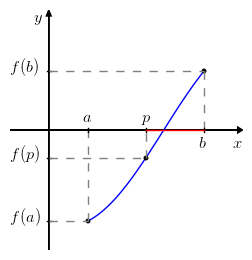
\includegraphics{./cap_equacao1d/pics/metodo_da_bissecao/metodo_da_bissecao}
  \caption{Método da bisseção.}
  \label{fig:bisection_scheme}
\end{figure}

Em outras palavras, seja $(a^{(0)},b^{(0)})=(a,b)$ o intervalo inicial e $p^{(0)}=\frac{a^{(0)}+b^{(0)}}{2}$ a aproximação inicial. Se $f(p^{(0)})\cdot f(a^{(0)})<0$, então $(a^{(1)},b^{(1)})=(a^{(0)},p^{(0)})$, caso contrário, $(a^{(1)},b^{(1)})=(p^{(0)},b^{(0)})$. A nova aproximação para a raiz é $p^{(1)}=\frac{a^{(1)}+b^{(1)}}{2}$. Esse procedimento produz uma sequência $p^{(n)}$ que converge para a raiz.

\begin{ex}Faça 5 iterações do método da bisseção para encontrar a raiz de $f(x)=x^3+5x^2-12$ utilizando $a^{(0)}=1$ e $b^{(0)}=2$.
$$
\begin{array}{|c|c|c|c|c|c|c|}
\hline
n&a^{(n)}&b^{(n)}&p^{(n)}&f(a^{(n)})&f(b^{(n)})&f(p^{(n)})\\
\hline
0&a^{(0)}=1&b^{(0)}=2&p^{(0)}=1,5&-6 &16&2,625  \\
\hline
1&a^{(1)}=1&b^{(1)}=p^1=1,5&p^{(1)}=1,25&-6 &2,625&-2,234375  \\
\hline
2&a^{(2)}=1,25&b^{(2)}=1,5&p^{(2)}=1,375&&&\\
\hline
3&&&&&&\\
\hline
4&&&&&&\\
\hline
5&&&&&&\\
\hline
\end{array}
$$

\ifisscilab
No console do Scilab, temos:
\begin{verbatim}
-->deff('y=f(x)','y = x^3 + 5*x^2 - 12')
-->//iteracao 0
-->a=1; b=2; p=(a+b)/2;
-->[a,b,p,f(a),f(b),f(p)]
 ans  =
    1.    2.    1.5  - 6.    16.    2.625  
-->//iteracao 1
-->b = p; p = (a+b)/2;
-->[a,b,p,f(a),f(b),f(p)]
 ans  =
    1.    1.5    1.25  - 6.    2.625  - 2.234375
\end{verbatim}
\fi
\end{ex}

Observe que a distância entre $p^{(0)}$ e a raiz $p^*$ não pode exceder metade do intervalo, ou seja $|p^{(0)}-p^*|\leq \frac{b-a}{2}$. Da mesma forma, o erro absoluto entre $p^{(1)}$ e $p^*$ é menor que $\frac{1}{4}$ do intervalo, isto é, $|p^{(1)}-p^*|\leq \frac{b-a}{2^2}$. De modo geral, o erro absoluto na iteração $n$ é estimado por
$$
|p^{(n)}-p^*|\leq \frac{b-a}{2^{n+1}},\qquad n\geq 1.
$$
Também, se $\epsilon_n:=|p^{(n)}-p^*|$, então vale:
$$
\epsilon_{n+1}\leq \frac{1}{2}\left(\epsilon_n\right)^1
$$
e, por isso, dizemos que o método da bisseção possui taxa de convergência linear. Um método com taxa de convergência super-linear satisfaz
$$
\epsilon_{n+1}\leq C\left(\epsilon_n\right)^m,
$$
onde $m>1$ e $C$ é uma constante.

\begin{ex}Determine quantas iterações são necessárias para encontrar a raiz de $f(x)=x^3+5x^2-12$ com uma precisão de $10^{-3}$, utilizando $a^{(0)}=1$ e $b^{(0)}=2$.

Observe que precisamos da seguinte desigualdade
$$
|p^{(n)}-p^*|\leq \frac{b-a}{2^{n+1}}= \frac{1}{2^{n+1}}\leq 10^{-3}.
$$
Assim,
$$
\log_{2}2^{-(n+1)}\leq \log_{2}10^{-3}
$$
ou seja,
$$
-(n+1)\log_{2}2\leq -3\log_2(10)\Rightarrow  n+1\geq 3\log_2(10)\approx 9,97\Rightarrow  n\approx 8,97
$$
Portanto, $n\geq 9$.
\end{ex}

\ifisscilab
\subsection{Código Scilab: método da bisseção}

O seguinte código é uma implementação no Scilab do algoritmo da bisseção. As variáveis de entrada são:
\begin{itemize}
\item \verb+f+ - função objetivo
\item \verb+a+ - extremo esquerdo do intervalo de inspeção $[a, b]$
\item \verb+b+ - extremo direito do intervalo de inspeção $[a, b]$
\item \verb+TOL+ - tolerância (critério de parada)
\item \verb+N+ - número máximo de iterações
\end{itemize}
A variável de saída é:
\begin{itemize}
\item \verb+p+ - aproximação da raiz de \verb+f+, i.e. $f(p) \approx 0$.
\end{itemize}

\verbatiminput{./cap_equacao1d/codes/metodo_da_bissecao/bissecao.sci}
\fi

\section*{Exercícios}

\begin{Exercise} Mostre que a equação do problema \ref{existe_unica} possui uma solução no intervalo $[1, v+1]$ para todo $v$ positivo. Dica: defina $f(x)=\ln(x)+x-\frac{1}{x}-v$  e considere a seguinte estimativa:
  \begin{equation*}
    f(v+1)=f(1)+\int_1^{v+1}f'(x)dx\geq -v+\int_1^{v+1}dx=0.  
  \end{equation*}
Use esta estimativa para iniciar o método de bisseção e obtenha o valor da raiz com pelo menos 6 algarismos significativos para $v=1, 2, 3, 4$ e $5$.
\end{Exercise}
\begin{Answer}
  \begin{tiny}
    $1,390054$; $1,8913954$; $2,4895673$; $3,1641544$; $3,8965468$    
  \end{tiny}
\end{Answer}

\begin{Exercise} Trace o gráfico e isole as três primeiras raízes positivas da função:
  \begin{equation*}
    f(x)=5\sin(x^2)-\exp\left({\frac{x}{10}}\right)  
  \end{equation*}
em intervalos de comprimento $0,1$.
\end{Exercise}
\begin{Answer}
  \begin{tiny}
    A primeira raiz se encontra no intervalo $(0,4, 0,5)$. A segunda raiz no intervalo $(1,7, 1,8)$. A terceira raiz se encontra no intervalo $(2,5, 2,6)$.    
  \end{tiny}
\end{Answer}

\begin{Exercise}Utilize o método da bisseção na equação $\sqrt{x}=\cos(x)$ para encontrar $p^{(4)}$ em $[a,b]=[0, 1]$.
\end{Exercise}

\begin{Exercise}[title=Estática] Considere o seguinte problema físico: uma plataforma está fixa a uma parede através de uma dobradiça cujo momento é dado por:
  \begin{equation*}
    \tau=k\theta,
  \end{equation*}
onde $\theta$ é angulo da plataforma com a horizontal e $k$ é uma constante positiva. A plataforma é feita de material homogêneo, seu peso é $P$ e sua largura é $l$. Modele a relação entre o ângulo $\theta$ e o peso $P$ próprio da plataforma. Encontre o valor de $\theta$ quando $l=1~\mbox{m}$, $P=200~\mbox{N}$, $k=50~\mbox{Nm}/\mbox{rad}$, sabendo que o sistema está em equilíbrio. Use o método da bisseção e expresse o resultado com 4 algarismos significativos.
\end{Exercise}
\begin{Answer}
  \begin{tiny}
    $k\theta=\frac{lP}{2}\cos(\theta)$ com $\theta\in (0, \pi/2)$; $1,030$.
  \end{tiny}
\end{Answer}

\begin{Exercise} Interprete a equação $\cos(x)=kx$ como o problema de encontrar a intersecção da curva $y=\cos(x)$ com $y=kx$. Encontre o valor positivo $k$ para o qual essa equação admite exatamente duas raízes positivas distintas.
\end{Exercise}
\begin{Answer}
  \begin{tiny}
    $k\approx 0,161228$
  \end{tiny}
\end{Answer}

\begin{Exercise} Considere a equação de Lambert dada por:
  \begin{equation*}
    xe^x= t,
  \end{equation*}
onde $t$ é um número real positivo. Mostre que esta equação possui uma única solução $x^*$ que pertence ao intervalo $[0, t]$. Usando esta estimativa como intervalo inicial, quantos passos são necessário para obter o valor numérico de $x^*$ com erro absoluto inferior a $10^{-6}$ quando $t=1$, $t=10$ e $t=100$ através do método da bisseção? Obtenha esses valores.
\end{Exercise}
\begin{Answer}
  \begin{tiny}
    $19$; $23$; $26$; $0,567143$; $1,745528$; $3,385630$
  \end{tiny}
\end{Answer}

\begin{Exercise}\label{prob_raiz_dupla} O polinômio $f(x)=x^4-4x^2+4$ possui raízes duplas em $\sqrt{2}$ e $-\sqrt{2}$. O método da bisseção pode ser aplicados a $f$? Explique.
\end{Exercise}

\begin{Exercise}[title=Eletrônica]\label{prob_diodo} O desenho abaixo mostra um circuito não linear envolvendo uma fonte de tensão constante, um diodo retificador e um resistor. Sabendo que a relação entre a corrente ($I_d)$ e a tensão ($v_d$) no diodo é dada pela seguinte expressão:
  \begin{equation*}
    I_d=I_R\left(\exp\left(\frac{v_d}{v_t}\right)-1\right),
  \end{equation*}
onde $I_R$ é a corrente de condução reversa e $v_t$, a tensão térmica dada por $v_t=\frac{kT}{q}$ com $k$, a constante de Boltzmann, $T$ a temperatura de operação e $q$, a carga do elétron. Aqui  $I_R=1pA=10^{-12}~\mbox{A}$, $T=300~\mbox{K}$. Escreva o problema como uma equação na incógnita $v_d$ e, usando o método da bisseção, resolva este problema com 3 algarismos significativos para os seguintes casos:
\end{Exercise}
\begin{minipage}[l]{0.6\linewidth}
\begin{itemize}
\item[a)] $V=30~\mbox{V}$ e $R=1~\mbox{k}\Omega$.
\item[b)] $V=3~\mbox{V}$ e $R=1~\mbox{k}\Omega$.
\item[c)] $V=3~\mbox{V}$ e $R=10~\mbox{k}\Omega$.
\item[d)] $V=300~\mbox{mV}$ e $R=1~\mbox{k}\Omega$.
\item[e)] $V=-300~\mbox{mV}$ e $R=1~\mbox{k}\Omega$.
\item[f)] $V=-30~\mbox{V}$ e $R=1~\mbox{k}\Omega$.
\item[g)] $V=-30~\mbox{V}$ e $R=10~\mbox{k}\Omega$.
\end{itemize}\end{minipage}\begin{minipage}[c]{0.4\linewidth}
\includegraphics[width=0.9\textwidth]{./cap_equacao1d/pics/circuito_diodo.eps}
\end{minipage}\\
Dica: $V=RI_d+v_d$.
\begin{Answer}
  \begin{tiny}
    a) $0,623$; b) $0,559$; c) $0,500$; d) $0,300$; e) $-0,3$; f) $-30$; g) $-30$
  \end{tiny}
\end{Answer}


\section{Iteração de Ponto Fixo}\index{iteração!do ponto fixo}

\subsection{Exemplo Histórico}
Vamos analisar o método babilônico para extração da raiz quadrada de um número positivo $A$ usando operações de soma, subtração, divisão e multiplicação.

Seja $x>0$ uma aproximação para $\sqrt{A}$, temos três caso:
\begin{itemize}
\item $x>\sqrt{A} \Longrightarrow \frac{A}{x}<\sqrt{A} \Longrightarrow \sqrt{A}\in \left(\frac{A}{x},x\right)$
\item $x=\sqrt{A} \Longrightarrow \frac{A}{x}=\sqrt{A}$
\item $x<\sqrt{A} \Longrightarrow \frac{A}{x}>\sqrt{A} \Longrightarrow \sqrt{A}\in \left(x,\frac{A}{x}\right)$
\end{itemize}
É natural imaginar que uma melhor aproximação para $\sqrt{A}$ é dada por
$$y=\frac{x+\frac{A}{x}}{2}$$

Aplicando esse método repetidas vezes, construímos a seguinte iteração:
\begin{eqnarray*}
x^{(n+1)}&=&\frac{x^{(n)}}{2}+\frac{A}{2x^{(n)}}\\
x^{(0)}&=&x
\end{eqnarray*}

\begin{ex}
A=5, x=2
\begin{eqnarray*}
x^{(n+1)}&=&\frac{x^{(n)}}{2}+\frac{2,5}{x^{(n)}}\\
x^{(0)}&=&2
\end{eqnarray*}

\begin{eqnarray*}
x^{(0)}&=&2\\
x^{(1)}&=&\frac{2}{2}+\frac{2,5}{2}=1+1,25=2,25\\
x^{(2)}&=&\frac{2,25}{2}+\frac{2,5}{2,25}= 2,2361111  \\
x^{(3)}&=&\frac{2,2361111}{2}+\frac{2,5}{2,2361111}= 2,236068  \\
x^{(4)}&=&\frac{2,236068}{2}+\frac{2,5}{2,236068}= 2,236068
\end{eqnarray*}  
\end{ex}

\begin{ex}
A=10, x=1
\begin{eqnarray*}
x^{(n+1)}&=&\frac{x^{(n)}}{2}+\frac{5}{x^{(n)}}\\
x^{(0)}&=&1
\end{eqnarray*}
\begin{eqnarray*}
x^{(0)}&=&1\\
x^{(1)}&=&\frac{1}{2}+\frac{5}{1}=0,5+5=5,5\\
x^{(2)}&=&\frac{5,5}{2}+\frac{5}{5,5}=3,6590909 \\
x^{(3)}&=&\frac{3,6590909}{2}+\frac{5}{3,6590909}=3,1960051   \\
x^{(4)}&=&\frac{3,1960051}{2}+\frac{5}{3,1960051}=3,1624556  \\
x^{(5)}&=&\frac{3,1624556}{2}+\frac{5}{3,1624556}=3,1622777  \\
x^{(6)}&=&\frac{3,1622777}{2}+\frac{5}{3,1622777}=3,1622777  \\
\end{eqnarray*}  
\end{ex}

A experimentação numérica sugere que o método funciona, mas três perguntas devem ser respondidas:
\begin{enumerate}
\item Será que a sequência é convergente?
\item Caso seja convergente, será que o limite $x^*=\lim_{n\to \infty }x_n$ é igual a $\sqrt{A}$?
\item Caso seja convergente, quão rápida é a convergência?
\end{enumerate}

A segunda pergunta é a mais fácil de ser respondida:

Supondo que o limite de $x_n$ exista, basta substituir na iteração:
\begin{eqnarray*}
\lim_{n \to \infty }x^{(n+1)}&=&\lim_{n \to \infty }\frac{x^{(n)}}{2}+\lim_{n \to \infty }\frac{A}{2x^{(n)}}\\
x^*&=&\frac{x^*}{2}+\frac{A}{2x^*}\\
\frac{x^*}{2}&=&\frac{A}{2x^*}\\
{x^*}&=&\frac{A}{x^*}\\
{(x^*)}^2&=&{A}\\
x^*&=&\sqrt{A}
\end{eqnarray*}
Portanto, sempre que esse método converge, temos a garantia de que o limite é $\sqrt{A}$. (Independente do valor inicial!)

De fato, podemos provar que o método é convergente para qualquer valor inicial positivo $x$. E, ainda, que a convergência é rápida (ainda precisamos definir isso).

Para responder essas perguntas, devemos formalizar o conceito de ponto fixo. Antes disso, analisemos mais um exemplo:

\subsection{Outro Exemplo}

Suponha que queiramos resolver a equação:
$$xe^x=10.$$
Observamos que o este problema é equivalente a resolver:
\begin{equation*}
x=\ln\left(\frac{10}{x}\right)  
\end{equation*}
ou:
\begin{equation*}
x=10e^{-x}
\end{equation*}

Para tanto, vamos propor os seguintes processos iterativos:

$$\begin{array}{l}
a)\left\{\begin{array}{ll}x^{(n+1)}=\ln\left(\frac{10}{x^{(n)}}\right),~~ n\geq 0\\
x^{(0)}=1
\end{array}\right.\\ \hbox{e} \\
b)\left\{\begin{array}{ll}x^{(n+1)}={10}{e^{-x^{(n)}}},~~ n\geq 0\\
x^{(0)}=1
\end{array}\right.\end{array}$$

O processo $a)$ produz a seguinte sequência:
\begin{eqnarray*}
x^{(0)}&=&1\\
x^{(1)}&=&\ln\left({10}\right)=2,3025851\\
x^{(2)}&=&\ln\left(\frac{10}{2,3025851}\right)=1,4685526\\
x^{(3)}&=&\ln\left(\frac{10}{1,4685526}\right)=1,9183078 \\
x^{(4)}&=&\ln\left(\frac{10}{1,9183078}\right)=1,6511417  \\
&\vdots&\\
x^{(10)}&=&1,7421335 \\
x^{(20)}&=& 1,7455151\\
x^{(30)}&=& 1,745528\\
x^{(31)}&=& 1,745528
\end{eqnarray*}

O processo $b)$ produz a seguinte sequência:
\begin{eqnarray*}
x^{(0)}&=&1\\
x^{(1)}&=&10e^{-1}= 3,6787944   \\
x^{(2)}&=&10e^{- 3,6787944 }= 0,2525340     \\
x^{(3)}&=&10e^{-0,2525340}=  7,7682979      \\
x^{(4)}&=&10e^{-7,7682979}=  0,0042293      \\
x^{(5)}&=&10e^{-0,0042293}=  9,9577961
\end{eqnarray*}


O experimento numérico sugere que o processo $a$ não é convergente e que o processo $b$ converge para $1,745528$.

\subsection{Ponto fixo}\index{ponto fixo}

Seja $\phi (x)$ uma função, dizemos que $x^*\in D(f)$ é um ponto fixo de $\phi$ se
$$\phi(x^*)=x^*$$

Seja $\phi:[a,b]\to [a,b]$ um função real tal que
$$|\phi(x)-\phi(y)|\leq \beta |x-y|,~~~\beta<1.$$
Então $\phi$ é dita uma contração e existe um único ponto $x^*\in [a,b]$ tal que $\phi(x^*)=x^*$. Além disso, a sequência
$$x^{(n+1)}=\phi(x^{(n)})$$
é convergente sempre que $x_0\in[a,b]$ e vale o limite $$\lim_{n\to\infty}x^{(n)}=x^*.$$

\begin{obs}
A desigualdade $|\phi(x)-\phi(y)|\leq \beta |x-y|$ implica que $\phi(x)$ é contínua.  
\end{obs}

Começamos demonstrando que existe pelo menos um ponto fixo. Para tal definimos a função $f(x)=x-\phi(x)$ e observamos que
$$f(a)=a-\phi(a)\leq a-a=0$$
e
$$f(b)=b-\phi(b)\geq b-b=0$$
Se $f(a)=a$ ou $f(b)=b$, então o ponto fixo existe. Caso contrário, as desigualdade são estritas e a função muda de sinal no intervalo. Como a função é contínua, pelo teorema do valor intermediário, existe um ponto $x^*$ no intervalo $(a,b)$ tal que $f(x^*)=0$, ou seja, $x^*-\phi(x^*)=0$. Observe que $x^*$ é um ponto fixo de $\phi$, pois $\phi(x^*)=x^*$. 

Para provar que o ponto fixo é único, observamos que se $x^*$ e $x^{**}$ são pontos fixos, eles devem ser iguais, pois:
$$|x^*-x^{**}|=|\phi(x^{*})-\phi(x^{**})|\leq \beta |x^*-x^{**}|$$
A desigualdade $|x^*-x^{**}|\leq \beta |x^*-x^{**}|$ com $\beta<1$ implica $|x^*-x^{**}|=0$.
\\~\\

Para demonstrar a convergência da sequência, observamos a seguinte relação
$$|x^{(n+1)}-x^*|=|\phi(x^{(n)})-x^*|=|\phi(x^{(n)})-\phi(x^*)|\leq \beta |x^{(n)}-x^*|.$$

Agora observamos que
$$|x^{(n)}-x^*|\leq  \beta |x^{(n-1)}-x^*|\leq \beta^2 |x^{(n-2)}-x^*|\leq \cdots \leq \beta^{n}|x^{(0)}-x^*|.$$
Portanto
$$\lim_{n\to\infty}|x^{(n)}-x^*|=0$$
e
$$\lim_{n\to\infty}x^{(n)}=x^*$$

Observações:
\begin{itemize}
\item A condição $|\phi(x)-\phi(y)|\leq \beta |x-y|$ é satisfeita sempre que $|\phi'(x)|\leq \beta<1$ em todo o intervalo pois
$$|\phi(x)-\phi(y)|=\left|\int_x^y\phi'(s)ds\right|\leq \int_x^y|\phi'(s)|ds\leq \int_x^y\beta ds=\beta|x-y|,~~ x<y.$$

\item A desigualdade estrita $\beta<1$ é necessária.

\item A condição $f([a,b])\subseteq [a,b]$ é necessária.

\end{itemize}


\subsection{Teste de convergência}
Seja $\phi :[a,b]$ uma função $C^0[a,b]$ e $x^*\in(a,b)$ um ponto fixo de $\phi$. Então $x^*$ é dito estável se existe uma região $(x^*-\delta,x^*+\delta)$ chamada bacia de atração tal que $x^{(n+1)}=\phi(x^{(n)})$ é convergente sempre que $x^{(0)}\in(x^*-\delta,x^*+\delta)$.

Teorema: Se $\phi\in C^1[a,b]$ e  $|\phi'(x^*)|<1$, então $x^*$ é estável. Se $|\phi'(x^*)|>1$ é instável e o teste é inconclusivo se $|\phi'(x^*)|=1$.


\begin{ex}
Considere o problema de encontrar a solução da equação algébrica
$$\cos(x)=x$$
vendo-a como o ponto fixo da função
$$f(x)=\cos(x).$$

Mostraremos que o teorema do ponto fixo se aplica a esta função com $[a,b]=[1/2,1]$.

Precisamos provar:
\begin{enumerate}
\item $f\left([1/2,1]\right) \subseteq [1/2,1]$;
\item $|f'(x)|<\beta,~~~\beta<1,~~~ \forall x\in [1/2,1]$.
\end{enumerate}

Para provar o item 1, observamos que $f(x)$ é decrescente no intervalo, pelo que temos:
$$0,54<\cos(1)\leq \cos(x)\leq \cos(1/2)<0,88$$
Como $[0,54,~0,88]\subseteq [0,5,~1]$, temos o item a.

Para provar o item 2, observamos que
$$f'(x)=-\sin(x)$$
Da mesma forma, temos a estimativa:
$$-0,85<-\sin(1) \leq -\sin(x)\leq -\sin(1/2)<-0,47$$
Assim, $|f'(x)|<0,85$ temos a desigualdade com $\beta=0,85<1$.

Agora, observamos o comportamento numérico da sequência:
$$\left\{\begin{array}{ll}x^{(n+1)}=\cos(x^{(n)}),~~ n\geq 0\\
x^{(0)}=1
\end{array}\right.$$


Os primeiros termos podem ser calculados numericamente e são dados por:
\begin{eqnarray*}
x^{(1)}&=&\cos(x_0)=\cos(1)=0,5403023\\
x^{(2)}&=&\cos(x_1)=\cos(0,5403023)=0,8575532\\
x^{(3)}&=&\cos(x_2)=\cos(0,8575532)=0,6542898\\
x^{(4)}&=&\cos(x_3)=\cos(0,6542898)=0,7934804\\
x^{(5)}&=&\cos(x_4)=\cos(0,7934804)=0,7013688\\
x^{(6)}&=&\cos(x_5)=\cos(0,7013688)=0,7639597\\
x^{(7)}&=&\cos(x_6)=\cos(0,7639597)=0,7221024\\
x^{(8)}&=&\cos(x_7)=\cos(0,7221024)=0,7504178\\
x^{(9)}&=&\cos(x_8)=\cos(0,7504178)=0,7314040\\
x^{(10)}&=&\cos(x_9)=\cos(0,7314040)= 0,7442374  \\
x^{(11)}&=&\cos(x_{10})=\cos(0,7442374)=0,7356047  \\
x^{(12)}&=&\cos(x_{11})=\cos(0,7356047)=0,7414251  \\
x^{(13)}&=&\cos(x_{12})=\cos(0,7414251)=0,7375069  \\
%x_{14}&=&\cos(x_{13})=\cos(0,7375069)=0,7401473  \\
&\vdots&\\
x^{(41)}&=&\cos(x_{40})=\cos(0,7390852)= 0,7390851  \\
x^{(42)}&=&\cos(x_{41})=\cos(0,7390851)= 0,7390851   \\
x^{(43)}&=&\cos(x_{42})=\cos(0,7390851 )= 0,7390851
\end{eqnarray*}
\end{ex}


\subsection{Estabilidade e convergência}\index{iteração do ponto fixo!estabilidade}\index{iteração do ponto fixo!convergência}

A fim de compreendermos melhor os conceitos de estabilidade e convergência, considere uma função $\Phi(x)$ com um ponto fixo $x^*=\phi(x^*)$ e analisemos o seguinte processo iterativo:
\begin{eqnarray*}
x^{(n+1)}&=&\phi\left(x^{(n)}\right)\\
x^{(0)}&=&x
\end{eqnarray*}
Vamos supor que a função $\phi(x)$ pode ser aproximada por seu polinômio de Taylor em torno do ponto fixo:
\begin{eqnarray*}
\phi(x)&=&\phi(x^*)+(x-x^*) \phi'(x^*)+O\left((x-x^*)^2\right), n\geq 0\\
&=&x^*+(x-x^*) \phi'(x^*)+O\left((x-x^*)^2\right)\\
&\approx& x^*+(x-x^*) \phi'(x^*)
\end{eqnarray*}

Substituindo na relação de recorrência, temos
$$
x^{(n+1)}=\phi\left(x^{(n)}\right)\approx x^*+(x^{(n)}-x^*) \phi'(x^*)
$$
Ou seja:
$$
\left(x^{(n+1)}-x^*\right)\approx {(x^{(n)}-x^*)} \phi'(x^*)
$$
Tomando módulos, temos:
$$
\underbrace{\left|x^{(n+1)}-x^*\right|}_{\epsilon_{n+1}}\approx \underbrace{\left|x^{(n)}-x^*\right|}_{\epsilon_n} \left|\phi'(x^*)\right|,
$$
onde $\epsilon_n=\left|x^{(n)}-x^*\right|$.

{\bf Conclusões:}
\begin{itemize}
\item Se $|\phi'(x^*)|<1$, então, a distância de $x^{(n)}$ até o ponto fixo $x^*$ está diminuindo a cada passo.
\item Se $|\phi'(x^*)|>1$, então, a distância de $x^{(n)}$ até o ponto fixo $x^*$ está aumentando a cada passo.
\item Se $|\phi'(x^*)|=1$, então, nossa aproximação de primeiro ordem não é suficiente para compreender o comportamento da sequência.
\end{itemize}

Fixaremos, portanto, nos casos quando $|\phi'(x^*)|<1$.

\subsection{Erro absoluto e tolerância}\index{erros!absoluto}\index{tolerência}

Na prática, quando se aplica uma iteração como esta, não se conhece de antemão o valor do ponto fixo $x^*$. Assim, o erro $\epsilon_n=\left|x^{(n)}-x^*\right|$ precisa ser estimado com base nos valores calculados $x^{(n)}$. Uma abordagem frequente é analisar a evolução da diferença entre dois elementos da sequência:
$$\Delta_n=\left|x^{(n+1)}-x^{(n)}\right|$$

A pergunta natural é: Será que o erro $\epsilon_n=\left|x^{(n)}-x^*\right|$ é pequeno quando  $\Delta_n=\left|x^{(n+1)}-x^{(n)}\right|$ for pequeno?

Para responder a esta pergunta, observamos que
$$x^*=\lim_{n\to \infty }x^{(n)}$$
portanto:
\begin{eqnarray*}
x^*-x^{(N)}&=&  \left(x^{(N+1)}-x^{(N)}\right)+\left(x^{(N+2)}-x^{(N+1)}\right)+\left(x^{(N+3)}-x^{(N+2)}\right)+\ldots\\
&=&\sum_{k=0}^\infty \left(x^{(N+k+1)}-x^{(N+k)}\right)
\end{eqnarray*}

Usamos também as expressões:
\begin{eqnarray*}
x^{(n+1)}&\approx& x^*+(x^{(n)}-x^*) \phi'(x^*)\\
x^{(n)}&\approx& x^*+(x^{(n-1)}-x^*) \phi'(x^*)
\end{eqnarray*}
Subtraindo uma da outra, temos:
\begin{eqnarray*}
x^{(n+1)}-x^{(n)}&\approx& (x^{(n)}-x^{(n-1)}) \phi'(x^*)
\end{eqnarray*}
Portanto:
\begin{eqnarray*}
x^{(N+k+1)}-x^{(N+k)}&\approx& (x^{(N+1)}-x^{(N)}) \left(\phi'(x^*)\right)^{k}
\end{eqnarray*}
%%%%%%%%%%%%%%%%%%%%%%%%%%%%
E temos:
\begin{eqnarray*}
x^*-x^{(N)}
&=&\sum_{k=0}^\infty \left(x^{(N+k+1)}-x^{(N+k)}\right)\\
&\approx&\sum_{k=0}^\infty (x^{(N+1)}-x^{(N)}) \left(\phi'(x^*)\right)^{k}\\
&=&(x^{(N+1)}-x^{(N)}) \frac{1}{1-\phi'(x^*)}, \left|\phi'(x^*)\right|<1
\end{eqnarray*}
Tomando módulo, temos:
\begin{eqnarray*}
\left|x^*-x^{(N)} \right|
&\approx&\left|x^{(N+1)}-x^{(N)}\right| \frac{1}{1-\phi'(x^*)}\\
\epsilon_N &\approx&  \frac{\Delta_N}{1-\phi'(x^*)}
\end{eqnarray*}

{\bf Conclusões:} Tendo em mente a relação $x^{(n+1)}-x^{(n)}  \approx (x^{(n)}-x^{(n-1)}) \phi'(x^*)$, concluímos:
\begin{itemize}
\item Quando $\phi'(x^*)<0$, o esquema é alternante e o erro $\epsilon_N$ pode ser estimado diretamente da diferença $\Delta_N$.
\item Quando $\phi'(x^*)>0$, o esquema é monótono e $\frac{1}{1-\phi'(x^*)}>1$, pelo que o erro $\epsilon_N$ é maior que a diferença $\Delta_N$. A relação será tão mais importante quando mais próximo da unidade for $\phi'(x^*)$, ou seja, quando mais lenta for a convergência.
\item Como $\phi'(x^*)\approx \frac{x^{(n+1)}-x^{(n)}}{x^{(n)}-x^{(n-1)}}$, temos
$$\left|\phi'(x^*)\right|\approx \frac{\Delta_n}{\Delta_{n-1}}$$
e portanto
$$\epsilon_N \approx \frac{\Delta_N}{1-\frac{\Delta_n}{\Delta_{n-1}}}.$$
\end{itemize}

\begin{obs}
  Deve-se exigir que $\Delta_n<\Delta_{n-1}$
\end{obs}

\section*{Exercícios}

\begin{Exercise}  Mostre que a equação:
  \begin{equation*}
    \cos(x)=x  
  \end{equation*}
possui uma única solução no intervalo $[0, 1]$. Encontre uma aproximação para esta solução com  4 dígitos significativos.
\end{Exercise}
\begin{Answer}
  \begin{tiny}
    $0,7391$
  \end{tiny}
\end{Answer}

\begin{Exercise} Verifique (analiticamente) que a única solução real da equação:
  \begin{equation*}
    xe^x=10
  \end{equation*}
é ponto fixo das seguintes funções:
\begin{itemize}
\item[a)] $\phi(x)=\ln\left(\frac{10}{x}\right)$
\item[b)] $\phi(x)=x-\frac{xe^{x}-10}{15}$
\item[c)] $\phi(x)=x-\frac{xe^{x}-10}{10+e^{x}}$
\end{itemize}
Implemente o processo iterativo $x^{(n+1)}=\phi(x^{(n)})$ para $n\geq 0$ e compare o comportamento. Discuta os resultados com base na teoria estudada.
\end{Exercise}

\begin{Exercise} Verifique (analiticamente) que a única solução real da equação:
  \begin{equation*}
    \cos(x)=x  
  \end{equation*}
é ponto fixo das seguintes funções:
\begin{itemize}
\item[a)] $\phi(x)=\cos(x)$
\item[b)] $\phi(x)=0,4 x+ 0,6\cos(x)$
\item[c)] $\phi(x)=x+\frac{\cos(x)-x}{1+\sin(x)}$
\end{itemize}
Implemente o processo iterativo $x^{(n+1)}=\phi(x^{(n)})$ para $n\geq 0$ e compare o comportamento.Discuta os resultados com base na teoria estudada.
\end{Exercise}


\begin{Exercise} Encontre a solução de cada equação com erro absoluto inferior a $10^{-6}$.
  \begin{itemize}
  \item[a)] $e^x=x+2$ no intervalo $(-2,0)$.
  \item[b)] $x^3+5x^2-12=0$ no intervalo $(1,2)$.
  \item[c)] $\sqrt{x}=\cos(x)$ no intervalo $(0,1)$.
  \end{itemize}
\end{Exercise}

\begin{Exercise} Encontre numericamente as três primeiras raízes positivas da equação dada por:
  \begin{equation*}
    \cos(x)=\frac{x}{10+x^2}  
  \end{equation*}
com erro absoluto inferior a $10^{-6}$.
\end{Exercise}

\begin{Exercise} Calcule uma equação da reta tangente a curva $y=e^{-(x-1)^2}$ que passa pelo ponto $(3, 1/2)$.
\end{Exercise}

\begin{Exercise} Resolva numericamente a inequação:
  \begin{equation*}
    e^{-x^2}<2x  
  \end{equation*}
\end{Exercise}
\begin{Answer}
  \begin{tiny}
    $x>a$ com $a\approx 0,4193648$.    
  \end{tiny}
\end{Answer}

\begin{Exercise} Considere os seguintes processos iterativos:
\begin{equation}
\begin{array}{l}
a\left\{\begin{array}{rcl}
x^{(n+1)}&=&\cos(x^{(n)})\\
x^{(1)}&=&.5
\end{array}
\right. \\ \qquad \hbox { e }\\
b\left\{\begin{array}{rcl}
x^{(n+1)}&=&.4x^{(n)}+.6\cos(x^{(n)})\\
x^{(1)}&=&.5
\end{array}
\right.
\end{array}
\end{equation}

Use o teorema do ponto fixo para verificar que cada um desses processos converge para a solução da equação $x^*$ de $\cos(x)=x$. Observe o comportamento numérico dessas sequências. Qual estabiliza mais rápido com cinco casas decimais? Discuta.

Dica: Verifique que $\cos([0.5,1])\subseteq [0.5,1]$ e depois a mesma identidade para a função $f(x)=.4x+.6\cos(x)$.
\end{Exercise}


\begin{Exercise}  Use o teorema do ponto fixo aplicado a um intervalo adequado para mostrar que a função $\phi(x)=\ln (100-x)$ possui um ponto fixo estável.
\end{Exercise}

\begin{Exercise}[title=Fluidos] Na hidráulica, o fator de atrito de Darcy é dado pela implicitamente pela equação de Colebrook-White:
$$\frac{1}{\sqrt{f}}= -2 \log_{10} \left( \frac{\varepsilon}{14.8 R_\mathrm{h}} + \frac{2.51}{\mathrm{Re}\sqrt{f}} \right)$$
onde $f$ é o fator de atrito, $\varepsilon$ é a rugosidade do tubo em metros, $R_\mathrm{h}$ é o raio hidráulico em metros e $\mathrm{Re}$ é o número de Reynolds. Considere $\varepsilon=2mm$, $R_\mathrm{h}=5cm$ e $\mathrm{Re}=10000$ e obtenha o valor de $f$ pela iteração:
$$x^{(n+1)}=-2 \log_{10} \left( \frac{\varepsilon}{14.8 R_\mathrm{h}} + \frac{2.51x^{(n)}}{\mathrm{Re}} \right)$$
\end{Exercise}
\begin{Answer}
  \begin{tiny}
$0.0431266$
  \end{tiny}
\end{Answer}

\begin{Exercise} Encontre uma solução aproximada para equação algébrica
$$180-100x=0.052\sinh^{-1}(10^{13}x)$$
com erro absoluto inferior a $10^{-3}$ usando um método iterativo.
Estime o erro associado ao valor de $v=180-100x=0.052\sinh^{-1}(10^{13}x)$, usando cada uma dessas expressões. Discuta sucintamente o resultado obtido. Dica: Este caso é semelhante ao problema \ref{prob_diodo}.
\end{Exercise}

\begin{Exercise}Considere que $x_n$ satisfaz a seguinte relação de recorrência:
$$x_{n+1}=x_n - \beta \left(x_n-x^*\right)$$
onde $\beta$ e $x^*$ são constantes.
Prove que $$x_n-x^*=(1-\beta)^{n-1}(x_1-x^*).$$
Conclua que $x_n\to x^*$ quando $|1-\beta|<1$.
\end{Exercise}

\begin{Exercise}[title=Convergência lenta] Considere o seguinte esquema iterativo:
$$
\left\{\begin{array}{l}
x^{(n+1)}=x_n+q^n\\
x^{(0)}=0
\end{array}
\right.$$
onde $q=1-10^{-6}$.
\begin{itemize}
\item[a)] Calcule o limite $$x_\infty=\lim_{n\to\infty}x^{(n)}$$ analiticamente.
\item[b)] Considere que o problema de obter o limite da sequência numericamente usando como critério de parada que $|x^{(n+1)}-x^{(n)}|<10^{-5}$. Qual o valor é produzido pelo esquema numérico? Qual o desvio entre o valor obtido pelo esquema numérico e o valor do limite obtido no item a?  Discuta. (Dica: Você não deve implementar o esquema iterativo, obtendo o valor de $x^{(n)}$ analiticamente)
\item[c)] Qual deve ser a tolerência especificada para obter o resultado com erro relativo inferior a $10^{-2}$?
\end{itemize}
\end{Exercise}

\begin{Exercise}[title=Convergência sublinear] Considere o seguinte esquema iterativo:
$$x^{(n+1)}=x^{(n)}-[x^{(n)}]^3,\ x^{(n)}\geq 0$$
com $x^{(0)}= 10^{-2}$.
Prove que $\{x^{(n)}\}$ é sequência de número reais positivos convergindo para zero. Verifique que são necessários mais de mil passos para que $x^{(n)}$ se torne menor que $0.9 x^{(0)}$.
\end{Exercise}


\begin{Exercise}[title=Taxa de convergência]
\begin{itemize}
\item[a)] Use o teorema do ponto fixo para mostrar que a função $\phi(x)=1-\sin(x)$ possui um único ponto fixo estável o intervalo $[\frac{1}{10},1]$. Construa um método iterativo $x^{(n+1)}=\phi(x^{(n)})$ para encontrar esse ponto fixo. Use o Scilab para encontrar o valor numérico do ponto fixo.
\item[b)] Verifique que função $\psi(x)=\frac{1}{2}\left[x+1-\sin(x)\right]$ possui um ponto fixo $x^*$ que também é o ponto fixo da função $\phi$ do item a. Use o Scilab para encontrar o valor numérico do ponto fixo através da iteração $x^{(n+1)}=\psi(x^{(n)})$. Qual método é mais rápido?
\end{itemize}
\end{Exercise}


\begin{Exercise}\it {(Esquemas oscilantes)}
\begin{itemize}
\item[a)] Considere a função $\phi(x)$ e função composta $\psi(x)=\phi\circ \phi=\phi\left(\phi(x)\right)$. Verifique todo ponto fixo de $\phi$ também é ponto fixo de $\psi$.

\item[b)]  Considere a função $$\phi(x)=10\exp(-x)$$ e função composta $\psi(x)=\phi\circ \phi=\phi\left(\phi(x)\right)$. Mostre que $\psi$ possui dois pontos fixos que não são pontos fixos de $\phi$.

\item[c)]  No problema anterior, o que acontece quando o processo iterativo $x^{(n+1)}=\phi(x^{(n)})$ é inicializado com um ponto fixo de $\psi$ que não é ponto fixo de $\phi$?
\end{itemize}
\end{Exercise}

\begin{Exercise}[title= Aceleração de convergência - introdução ao método de Newton]\label{int_new1} Mostre que se $f(x)$ possui uma raiz $x^*$ então a $x^*$ é um ponto fixo de $\phi(x)=x+\gamma(x) f(x)$. Encontre uma condição em $\gamma(x)$ para que o ponto fixo $x^*$ de $\phi$ seja estável. Encontre uma condição em $\gamma(x)$ para que $\phi'(x^*)=0$.
\end{Exercise}

\begin{Exercise}[title=Aceleração de convergência - introdução ao método de Newton]\label{int_new2} Considere que $x^{(n)}$ satisfaz a seguinte relação de recorrência:
$$x^{(n+1)}=x^{(n)} - \gamma f(x^{(n)})$$
onde $\gamma$ é uma constante. Suponha que $f(x)$ possui um zero em $x^*$. Aproxime a função $f(x)$ em torno de $x^*$ por
$$f(x)=f(x^*)+f'(x^*)(x-x^*)+O\left((x-x^*)^2\right).$$
Em vista do problema anterior, qual valor de $\gamma$ você escolheria para que a sequência $x^{(n)}$ convirja rapidamente para $x^*$. Que relação você encontra com o método de Newton?
\end{Exercise}

\begin{Exercise} Considere o problema da questão \ref{prob_diodo} e dois seguintes esquemas iterativos.
$$\begin{array}{l}
A\left\{
\begin{array}{ll}
I^{(n+1)}=\frac{1}{R}\left[V-v_t\ln\left(1+\frac{I^{(n)}}{I_R}\right)\right],n>0\\
I^{(0)}=0
\end{array}\right.\\ \hspace{2cm} \hbox{ e }\\
B\left\{
\begin{array}{ll}
I^{(n+1)}=I_R\left[\exp\left(\frac{V-RI^{(n)}}{v_t}\right)-1\right],n>0\\
I^{(0)}=0
\end{array}\right.
\end{array}
$$
Verifique numericamente que apenas o processo A é convergente para a, b e c; enquanto apenas o processo B é convergente para os outros itens.
\end{Exercise}

\section{Método de Newton-Raphson}\index{método de Newton-Raphson}

Consideramos o problema de encontrar as raízes da equação
$$f(x)=0$$ onde $f(x)\in C^1$ através do método do ponto fixo.
Para tal, observamos que um número real $x^*$ é raiz de $f(x)$ se e somente se $x^*$ é um ponto fixo da função
$$\phi(x)=x+\gamma(x)f(x), ~~\gamma(x)\neq 0$$
Aqui $\gamma(x)$ é uma função que será escolhida com base nos critérios de convergência do processo iterativo.


A derivada de $\phi(x)$ vale
$$\phi'(x)=1+\gamma(x)f'(x)+\gamma'(x)f(x)$$
no ponto $x^*$, temos
$$\phi'(x^*)=1+\gamma(x^*)f'(x^*)+\gamma'(x^*)f(x^*)$$
como $f(x^*)=0$, temos
$$\phi'(x^*)=1+\gamma(x^*)f'(x^*)$$

Sabemos que o processo iterativo converge tão mais rápido quanto menor for $\phi'(x)$ nas  vizinhanças de $x^*$, portanto, supomos que $f'(x^*)\neq 0$ e escolhemos $\gamma(x^*)$ de forma que
$$\phi'(x^*)=0,$$ ou seja
$$\gamma(x^*)=-\frac{1}{f'(x^*)}.$$

Observe que $x^*$ é raiz de $f(x)$ se, e somente se $x^*$ é ponto fixo de
$$\phi(x)=x-\frac{f(x)}{f'(x)}$$
e $\phi'(x^*)=0<1$. Portanto, o teorema do ponto fixo garante que se $x^{(0)}$ for suficientemente próximo a $x^*$, então o processo iterativo dado por
$$x^{(n+1)}=x^{(n)}-\frac{f(x^{(n)})}{f'(x^{(n)})}$$
converge para $x^*$, desde que $f'(x^{(n)})\neq 0 $ para todo $n\in\mathbb{N}$.

\subsection{Interpretação Geométrica}

Considere o problema de calcular a raiz uma função $f$, conforme esboço na figura abaixo

\begin{center}
\includegraphics[scale=.4]{./cap_equacao1d/pics/fig_Newton.eps}
\end{center}

Queremos calcular $x^{(1)}$ em função de $x^{(0)}$ sabendo que é o corte da reta tangente em $x^{(0)}$ com o eixo $x$. A equação da reta que passa por $(x^{(0)}, f(x^{(0)})$ e é tangente a curva em $x^{(0)}$ tem inclinação $m=f'(x^{(0)})$ e sua equação é
$$
y-f(x^{(0)})=f'(x^{(0)})(x-x^{(0)}).
$$
Sabendo que essa reta passa por $(x^{(1)},0)$, temos:
$$
0-f(x^{(0)})=f'(x^{(0)})(x^{(1)}-x^{(0)}).
$$
Portanto,
$$x^{(1)}=x^{(0)}-\frac{f(x^{(0)})}{f'(x^{(0)})}$$
que é uma iteração do método de Newton. Repetimos o processo para calcular $x^{(2)},\ x^{(3)},...$. De modo geral, temos:
$$x^{(n+1)}=x^{(n)}-\frac{f(x^{(n)})}{f'(x^{(n)})}.$$

\subsection{Análise de convergência}\index{método de Newton-Raphson!convergência}

Seja $f(x)$ um função com derivada e derivada segunda contínuas tal que $f(x^*)=0$ e $f'(x^*)\neq 0$. Seja também a função $\phi(x)$ definida como
$$\phi(x)=x-\frac{f(x)}{f'(x)}$$
Expandimos em série de Taylor em torno de $x^*$ e obtermos:
$$\phi(x)=\phi(x^*)+(x-x^*)\phi'(x^*)+ (x-x^*)^2\frac{\phi''(x^*)}{2}+O\left((x-x^*)^3\right)$$
Sabemos que
\begin{eqnarray*}
\phi(x^*)&=&x^*-\frac{f(x^*)}{f'(x^*)}=x^*\\
\phi'(x^*)&=&1-\frac{f'(x^*)f'(x^*)-f(x^*)f''(x^*)}{\left(f'(x^*)\right)^2}=1-1=0
\end{eqnarray*}
Portanto:
\begin{eqnarray*}
\phi(x)&=&x^*+ (x-x^*)^2\frac{\phi''(x^*)}{2}+O\left((x-x^*)^3\right)\\
&\approx&x^*+ (x-x^*)^2\frac{\phi''(x^*)}{2}.
\end{eqnarray*}
Logo,
\begin{eqnarray*}
x^{(n+1)}&=&\phi(x^{(n)})\\
&\approx& x^*+ (x^{(n)}-x^*)^2\frac{\phi''(x^*)}{2}
\end{eqnarray*}

\begin{eqnarray*}
\left(x^{(n+1)}-x^*\right) &\approx& (x^{(n)}-x^*)^2\frac{\phi''(x^*)}{2}
\end{eqnarray*}

\begin{obs} Pode-se mostrar facilmente que
$$\phi''(x^*)=\frac{f''(x^*)}{f'(x^*)}$$
\end{obs}

\section*{Exercícios}

\begin{Exercise} Considere o problema de calcular as soluções positivas da equação:
  \begin{equation*}
    \tg(x)=2x^2.    
  \end{equation*}
\begin{itemize}
\item[a)] Use o método gráfico para isolar as duas primeiras raízes positivas em pequenos intervalos. Use a teoria estudada em aula para argumentar quanto à existência e unicidade das raízes dentro intervalos escolhidos.
\item[b)] Calcule o número de iterações necessárias para que o método da bisseção aproxime cada uma das raízes com erro absoluto inferior a $10^{-8}$. Calcule as raízes por este método usando este número de passos.
\item[c)]  Calcule cada uma das raízes pelo método de Newton com oito dígitos significativos e discuta a convergência comparando com o item b).
\end{itemize}
{\bf Obs:} Alguns alunos encontraram como solução $x_1\approx 1,5707963$ e $x_2 \approx 4,7123890$. O que eles fizeram de errado?
\end{Exercise}
\ifisscilab
\begin{Answer}
  \begin{tiny}
    \begin{itemize}
\item[a)]Primeiramente, deve-se observar que a função $\tg(x)$ não está definida quando $x$ é um múltiplo ímpar de $\frac{\pi}{2}$, pelo que devemos cuidado nas singularidades. Traçamos o gráfico da função $f(x)=\tg(x)-2x^2$ no \verb+Scilab+ usando os seguintes comandos:
\begin{verbatim}
-->deff('y=f(x)','y=tan(x)-2*x^2')
-->plot([0:.01:1.3],f)
\end{verbatim} 
Observamos facilmente uma raiz no intervalo $(0,5, 0,6)$ e outra no intervalo $(1,2, 1,3)$. Como a função $f(x)$ é contínua fora dos pontos de singularidade da tangente, é fácil verificar que existe pelo menos uma solução nos intervalos dados pelo teorema do valor intermediário:
\begin{eqnarray*}
f(0,5) &\approx& 0,046302 >0\\
f(0,6) &\approx& -0,035863 <0\\
f(1,2) &\approx& -0,30784e-1 <0\\
f(1,3) &\approx&  0,22210e-1>0\\
\end{eqnarray*} 
Para provar a unicidade da solução em cada intervalo, precisamos mostra que a função é monótona, ou seja, a derivada não muda de sinal em cada intervalo:
\begin{eqnarray*}
f'(x)=\sec^2(x)-4x=\frac{1}{\cos^2(x)}-4x\leq \frac{1}{\cos^2(0,6)}-4*0,5<0, ~~x\in[ 0,5, 0,6]\\
f'(x)=\sec^2(x)-4x=\frac{1}{\cos^2(x)}-4x\geq \frac{1}{\cos^2(1,2)}-4*1,3>0, ~~x\in[ 1,2, 1,3]\\
\end{eqnarray*} 

\item[b)] 
Já isolamos as raízes em intervalos de comprimento $10^{-1}$ e a precisão requerida exige que as isolemos em intervalos de comprimento $2\times 10^{-8}$. Como cada passo da bisseção, confina a raiz em um intervalo com comprimento igual à metade do comprimento do intervalo anterior, temos a seguinte condição para o número de passos $N_p$:
$$\frac{10^{-1}}{2^N_p}\leq 2\times 10^{-8}$$
isso é equivalente a
$$N_p\geq \log_2 \frac{10^{-1}}{2\times 10^{-8}}=\log_2 \frac{10^{7}}{2}=7\log_2 10 -1=\frac{7}{\log_10 2}-1\approx 22.22$$
Como $N_p$ é inteiro, o menor $N_p$ que satisfaz a condição é $23$.

As raízes obtidas são $0.55970415$ e $1.2703426$. 

\item[c)] Para recalcular as raízes pelo método de Newton, basta executar a interação
$$x^{(n+1)}=x^{(n)}-\frac{f(x^{(n)})}{f'(x^{(n)}}$$    
\end{itemize}
Em relação à observação, o erro se deveu à falta de cuidado em compreender o problema antes de tentar resolvê-lo, em especial, à falta de observar que a função é descontínua em  múltiplos ímpares de $\frac{\pi}{2}$. Nestes pontos, a função $f(x)$ troca de sinal, mas não passa por zero.    
  \end{tiny}
\end{Answer}
\fi

\section*{Exercícios}

\ifisscilab
\begin{Exercise}\label{new1} Considere a equação
  $$e^{-x^2}=x$$
trace o gráfico com auxílio do \verb+Scilab+ e verifique que ela possui uma raiz positiva. Encontre uma aproximação para esta razão pelo gráfico e use este valor para inicializar o método de Newton e obtenha uma aproximação para a raiz com 8 dígitos significativos. (Use o comando \verb+format('v',16)+ para alterar a visualização no \verb+Scilab+.)
\end{Exercise}
\begin{Answer}
  \begin{tiny}
0,65291864    
  \end{tiny}
\end{Answer}
\fi

\begin{Exercise}\label{new2} Isole e encontre as cinco primeiras raízes positivas da equação com 6 dígitos corretos através de traçado de gráfico e do método de Newton.
$$\cos(10x)=e^{-x}.$$ Dica: a primeira raiz positiva está no intervalo $(0,0.02)$. Fique atento.
\end{Exercise}
\begin{Answer}
  \begin{tiny}
 $0.0198679$; $0.533890$; $0.735412$; $1.13237$; $1.38851$.
  \end{tiny}
\end{Answer}


\begin{Exercise}\label{new3} Encontre as raízes do polinômio $f(x)=x^4-4x^2+4$ através do método de Newton. O que você observa em relação ao erro obtido? Compare com a situação do problema \ref{prob_raiz_dupla}.
\end{Exercise}

\begin{Exercise}\label{new4} Encontre as raízes reais do polinômio $f(x)=\frac{x^5}{100}+x^4+3x+1$ isolando-as pelo método do gráfico e depois usando o método de Newton. Expresse a solução com 7 dígitos significativos.
\end{Exercise}
\begin{Answer}
  \begin{tiny}
$-99.99970$, $-0.3376513$; $-1.314006$.
  \end{tiny}
\end{Answer}

\begin{Exercise}Considere o método de Newton aplicado para encontrar a raiz de $f(x)=x^3-2x+2$. O que acontece quando $x^{(0)}=0$? Escolha um valor adequado para inicializar o método e obter a única raiz real desta equação.
\end{Exercise}

\begin{Exercise} Justifique a construção do processo iterativo do Método de Newton através do conceito de estabilidade de ponto fixo e convergência do método da iteração. Dica: Considere os problemas \ref{int_new1} e \ref{int_new2}.
\end{Exercise}

\begin{Exercise} Entenda a interpretação geométrica ao método de Newton. Encontre uma valor para iniciar o método de Newton aplicado ao problema $f(x)=xe^{-x}=0$ tal que o esquema iterativo divirja.
\end{Exercise}
\begin{Answer}
  \begin{tiny}
$x_0>1$.    
  \end{tiny}
\end{Answer}

\begin{Exercise}[title= Computação]Aplique o método de Newton à função $f(x)=\frac{1}{x}-u$ e construa um esquema computacional para calcular a inversa de $u$ com base em operações de multiplicação e soma/subtração.
 \end{Exercise}

\begin{Exercise}[title=Computação]Aplique o método de Newton à função $f(x)=x^n-A$ e construa um esquema computacional para calcular  $\sqrt[n]{A}$ para $A>0$ com base em operações de multiplicação e soma/subtração.
\end{Exercise}

\begin{Exercise} Considere a função dada por
\begin{eqnarray*}
\psi(x)&=&\ln\left(15-\ln(x)\right)
\end{eqnarray*}
definida para $x>0$
\begin{itemize}
\item [a)] (1.5) Use o teorema do ponto fixo para provar que se $x_0$ pertence ao intervalo $[1,3]$, então a sequência dada iterativamente por $$x^{(n+1)}=\psi(x^{(n)}),n\geq 0$$ converge para o único ponto fixo, $x^*$, de $\psi$. Construa a iteração $x^{(n+1)}=\psi(x^{(n)})$ e obtenha numericamente o valor do ponto fixo $x^*$. Expresse a resposta com 5 algarismos significativos corretos.
\item [b)] (1.0) Construa a iteração do método de Newton para encontrar $x^*$, explicitando a relação de recorrência e iniciando com $x_0=2$. Use o Scilab para obter a raiz e expresse a resposta com oito dígitos significativos corretos.
\end{itemize}
\end{Exercise}


\section{Método das Secantes}\index{método das secantes}

O Método das Secantes é semelhante ao Método de Newton. Neste método a derivada $f'(x)$ é aproximada pela declividade de um reta secante à curva:
$$f'(x)\approx \frac{f(x+\Delta x)-f(x)}{\Delta x}$$

Assim, em cada passo do método, calcula-se uma nova aproximação com base em duas aproximações anteriores:

$$x^{(n+1)}=x^{(n)} - \frac{f(x^{(n)})}{m}, \qquad m= \frac{f(x^{(n)})-f(x^{(n-1)})}{x^{(n)}-x^{(n-1)}} $$


\begin{ex} Encontre as raízes de $f(x)=\cos(x)-x$.\end{ex}

Da inspeção do gráfico das funções $y=\cos(x)$ e $y=x$, sabemos que esta equação possui uma raiz em torno de $x=0,8$. Iniciamos o método com $x_0=0,7$ e $x_1=0,8$.

\begin{center}
\begin{tabular}{|c|c|c|c|}\hline
$x^{(n-1)}$ & $x^{(n)}$ & $m$ & $x^{(n+1)}$\\\hline
 & & $\frac{f(0,8)-f(0,7)}{0,8-0,7} =$ & $0,8- \frac{f(0,8)}{-1,6813548}=$\\
$0,7$ & $0,8$ & $-1,6813548$ & $0,7385654$\\\hline
$0,8$ & $0,7385654$ & $-1,6955107$ & $0,7390784$ \\\hline
 $0,7385654$ & $0,7390784$ &  $-1,6734174$ & $0,7390851$ \\\hline
$0,7390784$ & $0,7390851$ & $-1,6736095$ & $0,7390851$ \\\hline
\end{tabular}  
\end{center}

\subsection{Análise de convergência}\index{método das secantes!convergência}

Seja $f(x)\in C^2$ um função tal que $f(x^*)=0$ e $f'(x^*)\neq 0$. Considere o processo iterativo do método das secantes:
$$x^{(n+1)}=x^{(n)}- \frac{f(x^{(n)})}{f(x^{(n)})-f(x^{(n-1)})}(x^{(n)}-x^{(n-1)})$$
Esta expressão pode ser escrita como:
\begin{eqnarray*}
x^{(n+1)}&=&x^{(n)}- \frac{f(x^{(n)})(x^{(n)}-x^{(n-1)})}{f(x^{(n)})-f(x^{(n-1)})}\\~\\
 &=&\frac{x^{(n)}\left(f(x^{(n)})-f(x^{(n-1)})\right)-f(x^{(n)})(x^{(n)}-x^{(n-1)})}{f(x^{(n)})-f(x^{(n-1)})}\\
 &=&\frac{x^{(n)} f(x^{(n-1)})-x^{(n-1)}f(x^{(n)})}{f(x^{(n)})-f(x^{(n-1)})}
\end{eqnarray*}

Subtraindo $x^*$ de ambos os lados temos:
\begin{eqnarray*}
x^{(n+1)}-x^*
 &=&\frac{x^{(n)} f(x^{(n-1)})-x^{(n-1)}f(x^{(n)})}{f(x^{(n)})-f(x^{(n-1)})}-x^*\\
 &=&\frac{x^{(n)} f(x^{(n-1)})-x^{(n-1)}f(x^{(n)})-x^*\left(f(x^{(n)})-f(x^{(n-1)})\right)}{f(x^{(n)})-f(x^{(n-1)})}\\
 &=&\frac{(x^{(n)}-x^*) f(x^{(n-1)})-(x^{(n-1)}-x^*)f(x^{(n)})}{f(x^{(n)})-f(x^{(n-1)})}
\end{eqnarray*}

Definimos $\epsilon_n=x_n-x^*$, equivalente a $x_n=x^*+\epsilon_n$
\begin{eqnarray*}
\epsilon_{n+1}
 &=&\frac{\epsilon_n f(x^*+\epsilon_{n-1})-\epsilon_{n-1}f(x^*+\epsilon_n)}{f(x^*+\epsilon_n)-f(x^*+\epsilon_{n-1})}
\end{eqnarray*}

Aproximamos a função $f(x)$ no numerador por
\begin{eqnarray*}
f(x^*+\epsilon)&\approx& f(x^*)+\epsilon f'(x^*) + \epsilon^2 \frac{f''(x^*)}{2}\\
f(x^*+\epsilon)&\approx& \epsilon f'(x^*) + \epsilon^2 \frac{f''(x^*)}{2}
\end{eqnarray*}

\begin{eqnarray*}
\epsilon_{n+1}
 &\approx&\frac{\epsilon_n \left[\epsilon_{n-1} f'(x^*) + \epsilon_{n-1}^2 \frac{f''(x^*)}{2}\right]-\epsilon_{n-1}\left[\epsilon_{n} f'(x^*) + \epsilon_{n}^2 \frac{f''(x^*)}{2}\right]}{f(x^*+\epsilon_n)-f(x^*+\epsilon_{n-1})}\\
~\\ &=&\frac{\frac{f''(x^*)}{2}\left(\epsilon_{n}\epsilon_{n-1}^2-\epsilon_{n-1}\epsilon_{n}^2\right)}{f(x^*+\epsilon_n)-f(x^*+\epsilon_{n-1})}\\
~\\ &=&\frac{1}{2}\frac{{f''(x^*)}\epsilon_{n}\epsilon_{n-1}\left(\epsilon_{n-1}-\epsilon_{n}\right)}{f(x^*+\epsilon_n)-f(x^*+\epsilon_{n-1})}
\end{eqnarray*}

Observamos, agora, que
\begin{equation}
  \begin{split}
  f(x^*+\epsilon_n)-f(x^*+\epsilon_{n-1}) &\approx \left[f(x^*)+f'(x^*)\epsilon_n\right]-\left[f(x^*)+f'(x^*)\epsilon_{n-1}\right] \\
  &=f'(x^*)(\epsilon_n-\epsilon_{n-1})  
  \end{split}  
\end{equation}

Portanto:
\begin{equation}
  \epsilon_{n+1}\approx \frac{1}{2}\frac{f''(x^*)}{f'(x^*)} \epsilon_n \epsilon_{n-1}
\end{equation}
ou, equivalentemente:
\begin{equation}
  x^{(n+1)}-x^*\approx \frac{1}{2}\frac{f''(x^*)}{f'(x^*)} \left(x^{(n)}-x^*\right) \left(x^{(n-1)}-x^*\right)
\end{equation}

Pode-se mostrar que
\begin{equation}
  |x^{(n+1)}-x^*|\approx M |x^{(n)}-x^*|^\phi,~~ n\hbox{ grande}
\end{equation}
com $\phi=\frac{\sqrt{5}+1}{2}\approx 1,618$ e $M$ é uma constante.


\begin{table}[h!]
  \centering
  \caption{Quadro comparativo.}
  \label{tab:quadro_comparativo}
  {\small
  \begin{tabular}[h!]{cccc} \hline
    Método & Convergência & Erro & Critério de parada \\ \hline
    \multirow{2}{*}{Bisseção} & Linear & \multirow{2}{*}{$\displaystyle \epsilon_{n+1}=\frac{1}{2}\epsilon$} & \multirow{2}{*}{$\displaystyle \frac{b_n - a_n}{2} < \text{erro}$} \\
    & ($p=1$) & & \\
    & & & \\
    Iteração & Linear & \multirow{2}{*}{$\displaystyle \epsilon_{n+1}\approx |\phi'(x^*)| \varepsilon_{n}$} & \multirow{2}{*}{$\displaystyle \begin{array}{cc} \frac{|\Delta_n|}{1-\frac{\Delta_n}{\Delta_{n-1}}}< \text{erro} \\ \Delta_{n} < \Delta_{n-1}\end{array}$} \\
    linear                 & ($p=1$) & & \\
    & & & \\
    \multirow{2}{*}{Newton} & Quadrática & \multirow{2}{*}{$\displaystyle \epsilon_{n+1}\approx \frac{1}{2}\left|\frac{f''(x^*)}{f'(x^*)}\right|\varepsilon_{n}^2$} & \multirow{2}{*}{$|\Delta_n|< \text{erro}$} \\
    & ($p=2$) & & \\
    & & & \\
    \multirow{3}{*}{Secante} & \multirow{3}{*}{$\displaystyle \begin{array}{rl} p &= {\displaystyle \frac{\sqrt{5}+1}{2}}\\
  &\approx 1,618\end{array}$} & \multirow{3}{*}{$\displaystyle \begin{array}{rl} \varepsilon_{n+1} &\approx \displaystyle \left|\frac{f''(x^*)}{f'(x^*)}\right| \varepsilon_{n}\varepsilon_{n-1} \\
    &\approx M \varepsilon_{n}^\phi\end{array}$} & \multirow{3}{*}{$|\Delta_n|< \text{erro}$}\\
    & & & \\
    & & & \\
    & & & \\ \hline
  \end{tabular}
}
\end{table}


\begin{obs}
O erro na tabela sempre se refere ao erro absoluto esperado. Nos três últimos métodos, é comum que se exija como critério de parada que a condição seja satisfeita por alguns poucos passos consecutivos. Outros critérios podem ser usados. No métodos das secantes, deve-se ter o cuidado de evitar divisões por zero quando $x_{n+1}-x_n$ muito pequeno em relação à resolução do sistema de numeração.  
\end{obs}

\section*{Exercícios}

\begin{Exercise} Refaça as questões \ref{new1}, \ref{new2}, \ref{new3}  e \ref{new4}, usando o método das secantes.
\end{Exercise}

\begin{Exercise} Dê uma interpretação geométrica ao método das secantes. Qual a vantagem do método das secantes sobre o método de Newton?
\end{Exercise}

\begin{Exercise} Aplique o método das secantes para resolver a equação
  \begin{equation*}
    e^{-x^2}=2x  
  \end{equation*}
\end{Exercise}

\begin{Exercise} Refaça o problema \ref{prob_diodo} usando o método de Newton e das secantes.
\end{Exercise}

\section*{Exercícios finais}

\begin{Exercise} A equação $$\cos(\pi x)=e^{-2x}$$ tem infinitas raízes.
Usando  métodos numéricos encontre as primeiras raízes dessa equação. Verifique a j-ésima raiz ($z_j$) pode ser aproximada por $j-1/2$ para $j$ grande. Use o método de Newton para encontrar uma aproximação melhor para $z_j$.
\end{Exercise}
\begin{Answer}
  \begin{tiny}
 $z_1\approx 0.3252768 $, $z_2\approx 1.5153738$, $z_3\approx 2.497846  $, $z_4\approx 3.5002901$, $z_j\approx j-1/2-(-1)^j\frac{e^{-2j+1}}{\pi}, ~~~j>4$    
  \end{tiny}
\end{Answer}


\begin{Exercise}[title=Eletricidade]A corrente elétrica, $I$, em Ampères em uma lâmpada em função da tensão elétrica, $V$, é dada por
$$I=\left(\frac{V}{150}\right)^{0.8}$$
Qual a potência da lâmpada quando ligada em série com uma resistência de valor R a uma fonte de 150V quando. (procure erro inferior a 1\%)
\begin{itemize}
\item [a)] $R=0\Omega$
\item [b)] $R=10\Omega$
\item [c)] $R=50\Omega$
\item [d)] $R=100\Omega$
\item [E)] $R=500\Omega$
\end{itemize}
\end{Exercise}
\begin{Answer}
  \begin{tiny}
$150$~W, $133$~W, $87$~W, $55$~W, $6,5$~W    
  \end{tiny}
\end{Answer}

%\begin{Exercise} Determine com 3 algarismos signficativos o valor de $R$ para que a potência na lâmpada seja $75W$ na questão anterior?

%Resp: $ 65.2\Omega$
%\end{Exercise}


\begin{Exercise} (Bioquímica) A concentração sanguínea de um medicamente é modelado pela seguinte expressão
$$c(t)=Ate^{-\lambda t}$$
onde $t>0$ é o tempo em minutos decorrido desde a administração da droga. $A$ é a quantidade administrada em $mg/ml$ e $\lambda$ é a constante de tempo em min$^{-1}$.
Responda:
\begin{itemize}
\item[a)] Sendo $\lambda=1/3$, em que instantes de tempo a concentração é metade do valor máximo. Calcule com precisão de segundos.
\item[b)] Sendo $\lambda=1/3$ e $A=100mg/ml$, durante quanto tempo a concentração permanece maior que $10mg/ml$.
\end{itemize}
\end{Exercise}

\begin{Answer}
  \begin{tiny}
a) $42$~s e $8$~min$2$~s, b) $14$~min$56$~s.    
  \end{tiny}
\end{Answer}


\begin{Exercise}\label{pop} Considere o seguinte modelo para crescimento populacional em um país:
$$P(t)=A+Be^{\lambda t}.$$
onde $t$ é dado em anos. Use $t$ em anos e $t=0$ para 1960. Encontre os parâmetros $A$, $B$ e $\lambda$ com base nos anos de 1960, 1970 e 1991 conforme tabela:\\~

\begin{tabular}{|c|c|}
\hline
Ano & população\\
\hline
1960&70992343\\
1970&94508583\\
1980&121150573\\
1991&146917459\\
\hline	
\end{tabular}

Use esses parâmetros para calcular a população em 1980 e compare com o valor do censo.
\end{Exercise}
\begin{Answer}
  \begin{tiny}
$118940992$
  \end{tiny}
\end{Answer}

\begin{Exercise}[title=Fluidos]\label{boiaesf} Uma boia esférica flutua na água. Sabendo que a boia tem $10\ell$ de volume e 2Kg de massa. Calcule a altura da porção molhada da boia.
\end{Exercise}
\begin{Answer}
  \begin{tiny}
$7,7$~cm    
  \end{tiny}
\end{Answer}

\begin{Exercise}[title= Fluidos]\label{boiacil} Uma boia cilíndrica tem secção transversal circular de raio 10cm e comprimento 2m e pesa 10Kg. Sabendo que a boia flutua sobre água com o eixo do cilindro na posição horizontal, calcule a altura da parte molhada da boia.
\end{Exercise}
\begin{Answer}
  \begin{tiny}
$4,32$~cm    
  \end{tiny}
\end{Answer}

\begin{Exercise} Encontre com 6 casas decimais o ponto da curva $y=\ln x$ mais próximo da origem.
\end{Exercise}
\begin{Answer}
  \begin{tiny}
$(0,652919, 0,426303)$    
  \end{tiny}
\end{Answer}


\begin{Exercise}[title= Matemática financeira] Um computador é vendido pelo valor a vista de R\$2.000,00 ou em 1+15 prestações de R\$200,00. Calcule a taxa de juros associada à venda a prazo.
\end{Exercise}

\begin{Answer}
  \begin{tiny}
$7,19$\% ao mês    
  \end{tiny}
\end{Answer}

\begin{Exercise}[title= Matemática financeira] O valor de R\$110.000,00 é financiado conforme a seguinte programa de pagamentos:

\begin{tabular}{|c|c|}
\hline
Mês & pagamento\\
\hline
1&20.000,00\\
2&20.000,00\\
3&20.000,00\\
4&19.000,00\\
5&18.000,00\\
6&17.000,00\\
7&16.000,00\\
\hline	
\end{tabular}

Calcule a taxa de juros envolvida. A data do empréstimo é o mês zero.
 \end{Exercise}

\begin{Answer}
  \begin{tiny}
$4,54$\% ao mês.    
  \end{tiny}
\end{Answer}


\begin{Exercise}[title=Controle de sistemas]  Depois de acionado um sistema de aquecedores, a temperatura em um forno  evolui conforme a seguinte equação
$$T(t)=500-800e^{-t}+600e^ {-t/3}.$$
onde $T$ é a temperatura em Kelvin e $t$ é tempo em horas.
\begin{itemize}
\item[a)] Obtenha analiticamente o valor de $\lim_{t\to\infty}T(t)$.
\item[b)] Obtenha analiticamente o valor máximo de $T(t)$ e o instante de tempo quando o máximo acontece
\item[c)] Obtenha numericamente com precisão de minutos o tempo decorrido até que a temperatura passe pela primeira vez pelo valor de equilíbrio obtido no item a.
\item[c)] Obtenha numericamente com precisão de minutos a duração do período durante o qual a temperatura permanece pelo menos 20\% superior ao valor de equilíbrio.
\end{itemize}
\end{Exercise}

\begin{Answer}
  \begin{tiny}
$500$~K, $700$~K em $t=3\ln(2)$, $26$~min, $4$~h$27$~min.    
  \end{tiny}
\end{Answer}

\begin{Exercise} Encontre os pontos onde a elipse que satisfaz $\frac{x^2}{3}+y^2=1$ intersepta a parábola $y=x^2-2$.
\end{Exercise}
\begin{Answer}
  \begin{tiny}
$\left(\pm 1,1101388, -0,7675919\right)$, $\left(\pm 1,5602111, 0,342585\right)$
  \end{tiny}
\end{Answer}

\begin{Exercise}[title= Otimização] Encontre a área do maior retângulo que é possível inscrever entre a curva $e^{-x^2}\left(1+\cos(x)\right)$ e o eixo $y=0$.
\end{Exercise}
\begin{Answer}
  \begin{tiny}
$1,5318075$
  \end{tiny}
\end{Answer}


\begin{Exercise}[title=Otimização] \label{usinas} Uma indústria consome energia elétrica de duas usinas fornecedoras. O custo de fornecimento em reais por hora como função da potência consumida em $kW$ é dada pelas seguintes funções
\begin{eqnarray*}
C_1(x)&=& 500+.27 x + 4.1\cdot 10^{-5}x^2 +2.1\cdot 10^{-7}x^3+4.2\cdot 10^{-10}x^4 \\
C_2(x)&=& 1000+.22 x + 6.3\cdot 10^{-5}x^2 +8.5\cdot 10^{-7}x^3
\end{eqnarray*}
Onde $C_1(x)$ e $C_2(x)$ são os custos de fornecimento das usinas 1 e 2, respectivamente. Calcule o custo mínimo da energia elétrica quando a potência total consumida é  $1500kW$.

\end{Exercise}
\begin{Answer}
  \begin{tiny}
 Aproximadamente 2500 reais por hora.    
  \end{tiny}
\end{Answer}

\begin{Exercise}[title= Termodinâmica] A pressão de saturação (em bar) de um dado hidrocarboneto pelo ser modelada pela equação de Antoine:
$$\ln\left(P^{sat}\right)=A-\frac{B}{T+C}$$
onde $T$ é a temperatura e $A$, $B$ e $C$ são constantes dadas conforme a seguir:

\begin{tabular}{|c|c|c|c|}
\hline
Hidrocarboneto&A&B&C\\
\hline
N-pentano & 9.2131 & 2477.07 & -39.94 \\
\hline
N-heptano & 9.2535 &2911.32 &-56.51 \\
\hline
\end{tabular}
\begin{itemize}
\item[a)] Calcule a temperatura de bolha de uma mistura de N-pentano e N-heptano à pressão de 1.2bar quando as frações molares  dos gases são  $z_1=z_2=0.5$. Para tal utilize a seguinte equação:
$$P=\sum_i z_i P_i^{sat}$$
\item[b)] Calcule a temperatura de orvalho de uma mistura de N-pentano e N-heptano à pressão de 1.2bar quando as frações molares  dos gases são  $z_1=z_2=0.5$. Para tal utilize a seguinte equação:
$$\frac{1}{P}=\sum_i \frac{z_i}{P_i^{sat}}$$
\end{itemize}
\end{Exercise}

\begin{Answer}
  \begin{tiny}
 a) $332,74$~K b) $359,33$~K    
  \end{tiny}
\end{Answer}

\begin{Exercise} Encontre os três primeiros pontos de mínimo da função $$f(x)=e^{-x/11}+x\cos(2x)$$ para $x>0$ com erro inferior a $10^{-7}$.
\end{Exercise}
\begin{Answer}
  \begin{tiny}
$1,2285751$, $4,76770758$, $7,88704085$
  \end{tiny}
\end{Answer}


%\end{document} 
